\chapter{Analisi} \label{analisi}

In questo capitolo verranno illustrati gli elementi fondamentali dell'ambiente di simulazione sviluppato.
Di seguito è possibile osserverne una rapida descrizione:

\begin{itemize}
    \item \textit{Ambiente:} area di esplorazione in cui sono posizionati tutti gli elementi;
    \item \textit{UAV:} entità incaricata di completare il task prefissato dalla missione;
    \item \textit{Target:} entità che rappresenta l'obiettivo della missione;
    \item \textit{Ostacolo:} entità che dev'essere rilevata dallo sciame di UAV;
    \item \textit{Algoritmo bio-ispirato:} strategia integrata nell'ambiente di simulazione contenente i vari meccanismi di coordinamento dello sciame.

\end{itemize}

\section{Ambiente}

L'ambiente rappresenta l'area bidimensionale all'interno della quale lo sciame è vincolato a muoversi.
L'ambiente risulta discretizzato sia da un punto di vista spaziale che temporale e può essere caratterizzato da obiettivi sia statici che dinamici, in base alla tipologia di missione.
La posizione degli obiettivi e degli ostacoli all'interno di quest'area bidimensionale dipende dallo scenario reale utilizzato durante la fase di simulazione.

\section{UAV: Unmanned Aerial Vehicles}

Quando parliamo di UAV - spesso chiamati droni - ci riferiamo alle uniche entità in grado di muoversi in maniera continua all'interno dell'ambiente di esplorazione.
Talì entità sono gli attori principali per il completamento della missione: l'organizzazione dipende dall'algoritmo integrato nel simulatore.
In generale, il task primario è quello di trovare tutti i target nel minor tempo possibile oppure di trovare il maggior numero possibile di target entro il tempo di autonomia della batteria, evitando sia gli ostacoli che gli altri UAV.
Si assume che i droni non conoscano la struttura dell'ambiente e, di conseguenza, non hanno informazioni sulla posizione degli altri UAV impiegati nella missione.
Il movimento all'interno dell'area e il coordinamento dello sciame è dettato dall'informazione feromonica rilasciata nell'ambiente e, naturalmente, dalla strategia utilizzata nell'algoritmo bioispirato utilizzato.

\subsection{Stati di un UAV} \label{stati}

Durante lo svolgimento di una missione, ogni UAV può assumere uno dei seguenti stati:

\begin{itemize}
    \item \textit{Explorer:} un drone che si trova in stato di esplorazione ha lo scopo di saggiare l'area alla ricerca di target;
    \item \textit{Coordinator:} nel caso in cui la missione lo preveda, il primo UAV ad identificare un targeti diventa coordinatore. Un attore in questo stato ha il compito di richiamare altri droni per intervenire sul target, in accordo con il task previsto dalla missione;
    \item \textit{Recruited:} nel caso in cui la missione lo preveda, un drone che si trova in stato di esplorazione può essere richiamato da un coordinatore per intervenire sul target, modificando il proprio stato in \textit{reclutato}, in accordo con il task previsto dalla missione;
    \item \textit{Waiting:} il numero di UAV necessari all'esecuzione di un target dipende dalla missione. Un drone reclutato, che ha raggiunto il coordinatore, modifica il proprio e resta in attesa che tale numero venga raggiunto;
    \item \textit{Execution:} una volta raggiunto il numero minimo di UAV per intervenire sul target, tutti i droni nell'area del target, coordinatore compreso, modifica il proprio stato per \textit{eseguire} il target, in accordo con il task previsto dalla missione.
\end{itemize}

Ogni algoritmo, integrato nel relativo modulo, può prevedere tutti gli stati o un subset di essi.
Nelle prossime sezioni saranno definiti, nel dettaglio, i possibili stati che un drone può assumere negli algoritmi presi in esempio.

\begin{figure}[H] 
    \captionsetup{justification=centering, margin=2cm, font=footnotesize}
    \begin{center}
    \makebox[\textwidth]{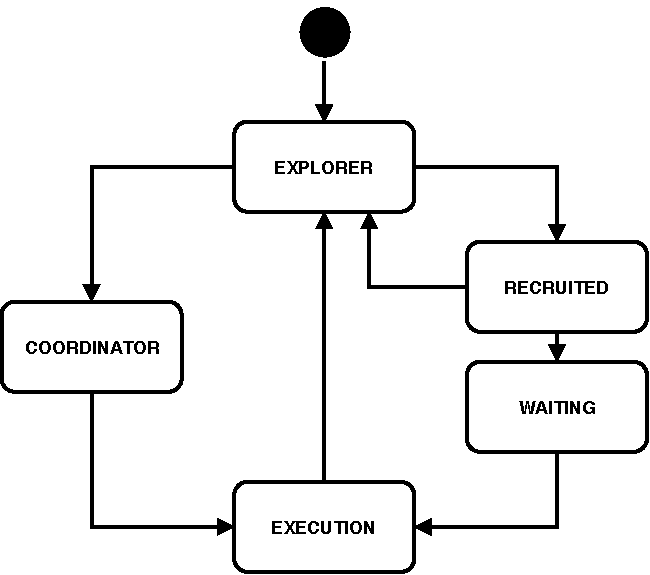
\includegraphics[width=0.3\paperwidth]{img/uav_states.pdf}}
    \end{center}
    \caption{Possibili stati di un drone}
    \label{uav_states}
\end{figure}

\section{Target}

I target si trovano in posizioni sconosciute a priori e devono essere scoperti e, se la missione lo prevede, eseguiti dai droni entro il loro tempo di autonomia.
Un target può essere, dunque, considerato come \textit{trovato} (found) quando un drone, equipaggiato con una tecnologia di sensing adeguata, si trova in una posizione tale da poterlo rilevare.
Un target è da considerare \textit{eseguito} (executed) nel momento in cui un subset dello sciame ha terminato la fase di esecuzione prevista dalla missione. \\
Alcuni esempi di target potrebbero essere:

\begin{itemize}
    \item mine antiuomo inesplose;
    \item discariche abusive;
    \item principi di incendi;
    \item \dots
\end{itemize}

\section{Ostacolo}

Un ostacolo è definito come un'entità statica all'interno dell'ambiente di simulazione, che non può essere attraversata dai droni.
Costruzioni e alberi rappresentano tipici esempi di ostacoli che possono trovarsi all'interno di un contesto applicativo.
Il numero, la forma e la dimensione degli ostacoli dipendono dalla quota di volo di un UAV: tipicamente, maggiore è la quota di volo e minore sarà il numero di ostacoli.

\section{Algoritmo bioispirato}

In questa sezione verranno esaminati alcuni punti chiave fondamentali che caratterizzano tipicamente gli algoritmi bioispirati, oggetto di comparazione all'interno dell'ambiente di simulazione.
Per semplificare la comprensione di tali meccanismi, verranno analizzati alcuni algoritmi presenti in letteratura che sono stati integrati all'interno del simulatore per un'analisi comparativa delle performance. 

\subsection{SFE-RR}

La strategia SFE-RR (\textit{Stigmergy-Flocking-Evolution for robots recruitment}) integrata all'interno del simulatore è stata inizialmente adottata dal simulatore SFE, pubblicamente rilasciato da Cimino et al. \cite{cimino2019adaptive}.
Nella sezione successiva verranno analizzati i meccanismi fondamentali di questa strategia, mentre nei capitoli successivi approfondiremo le novità introdotte nel nuovo ambiente.

Le metaeuristiche analizzate sono:

\begin{itemize}
    \item \textit{Collision avoidance};
    \item \textit{Stigmergia};
    \item \textit{Flocking};
\end{itemize}

\subsubsection{Modulo di collision avoidance}

Tipicamente, come già anticipato, l’ambiente di esplorazione prevede la presenza di ostacoli. 
Il numero di droni utilizzati per il completamento della missione, inoltre, potrebbe essere elevato.
Di conseguenza, risulta strettamente necessario un meccanismo di collision avoidance al fine di rendere più realistica la simulazione. 
Il modulo di collision avoidance può essere suddiviso in due sottomoduli:

\begin{enumerate}
    \item \textit{Modulo di obstacle avoidance:} l’obiettivo principale di questo modulo software è quello di evitare le collisioni tra i droni e gli ostacoli presenti nell’ambiente di esplorazione. 
    In un contesto applicativo reale, questo meccanismo risulta strettamente necessario per ragioni di sicurezza e di costi;
    \item \textit{Modulo di overlap avoidance:} l’obiettivo di questo modulo è quello di evitare che si verifichino collisioni (o scontri) tra due o più droni in movimento. 
    Questa condizione deve essere sempre verificata, in particolare quando il numero di droni dello sciame aumenta.
\end{enumerate}

\subsubsection{Stigmergia}

La stigmergia è un meccanismo bio-ispirato usato da formiche, api ed altri insetti sociali, ad esempio durante l’attività di foraggiamento. 
La stigmergia è un meccanismo emergente, perché entità con limitate capacità computazionali possono organizzarsi in maniera distribuita e robusta.

L’elemento fondamentale della stigmergia è il feromone, ovvero una sostanza chimica in grado di attrarre altre entità nei luoghi in cui viene rilasciata. 
Il feromone ha una durata limitata nel tempo e dopo un certo periodo scompare a causa dell’evaporazione. 
Inoltre, un’entità attratta dal feromone è soggetta all’assuefazione olfattiva: dopo un certo tempo l’attrazione esercitata dal feromone perde il suo effetto.

Il meccanismo di stigmergia, così come descritto, è stato progettato, implementato e testato nel simulatore SFE. 
Lo scopo principale è quello di attrarre altre entità su un target di interesse comune, perché, in questo modo, altri target vicini possono essere facilmente scoperti.

Il feromone può essere anche repulsivo: invece di attrarre entità in un’area delimitata, respinge le entità vicine.

\subsubsection{Flocking}

Il flocking è il comportamento esibito quando un gruppo di uccelli, denominato flock, sta facendo attività di foraggiamento oppure è in volo. 
Il flocking è simile al comportamento di shoaling dei pesci, al comportamento di swarming degli insetti e ai comportamenti di altri animali sociali. 
La ragione principale per organizzare le entità in flocks sta nel fatto di raggrupparle per rendere più efficiente ed affidabile il processo di scoperta dei target. 
Infatti, un flock costituito da più droni ha un raggio di sensing più ampio rispetto al singolo drone. 
Il meccanismo di flocking può essere ulteriormente suddiviso in tre diversi sotto-meccanismi:

\begin{enumerate}
    \item \textit{Separazione:} il meccanismo di separazione ha l'obiettivo di distanziare i droni, sia per prevenire le collisioni, sia per avere dei flock più ampi così da incrementare la copertura dell'area di sensing;
    \item \textit{Allineamento:} il meccanismo di allineamento ha lo scopo di allineare il drone nella direzione media del flock al fine di seguire in modo più accurato gli altri droni della stessa flotta;
    \item \textit{Coesione:} questo meccanismo ha lo scopo di recuperare il flock e si attiva quando un’entità è “troppo lontana” dal resto dei compagni. 
    Tale lontananza rappresenta un parametro regolabile all'interno del simulatore.
\end{enumerate}

\subsubsection{Stati di un drone}

Nell'ultima versione dell'algoritmo è stato introdotto un meccanismo che prevede la modifica dello stato del drone, in accordo con determinati eventi che si scatenano durante lo svolgimento della missione.
Nel caso specifico, un drone può assumere uno dei seguenti stati, che verranno illustrati in dettaglio nella fase di progettazione:
\begin{itemize}
    \item \textit{Explorer};
    \item \textit{Waiting};
    \item \textit{Execution};
\end{itemize}
Se la missione prevede una lavorazione del target, infatti, è necessario che un numero minimo di droni raggiunga una posizione relativamente vicina all'obiettivo.
In questo caso, parliamo di \textit{esecuzione del target}.

\subsection{Algoritmi di esplorazione e recruitment}

Gli autori in \cite{palmieri2017comparison} si sono concentrati sull'applicazione di diverse metaeuristiche di ispirazione biologica per il coordinamento di uno sciame che deve esplorare un'area sconosciuta al fine di trovare e gestire in modo cooperativo alcuni obiettivi distribuiti.
Di seguito verranno analizzate prima le metaeuristiche orientate all'esplorazione dell'area e successivamente quelle inerenti il coordinamento dello sciame per la gestione dei target identificati.

In questo caso, un agente può assumere tutti e 5 gli stati descritti nella sezione \ref{stati}.

\subsubsection{Esplorazione}

L'obiettivo della strategia di esplorazione è quello di visitare l'area d'interesse della missione in maniera efficiente, minimizzando la possibilità che gli attori visitino più volte una stessa area della regione.
A tal fine viene utilizzata una comunicazione basata sull'ambiente (\textit{stigmergia}) ed in particolare viene utilizzato un meccanismo feromonico repulsivo.
Durante l'esplorazione, il feromone viene depositato dal drone non appena si raggiunge la nuova cella. 
In questo modo, l'entità in movimento selezionerà la cella, appartenente al subset di celle immediatamente vicine alla posizione corrente, che presenta la traccia feromonica meno intensa.

L'uso dei feromoni è simile a quello del metodo \textit{Ant Colony Optimization}, ma a differenza delle formiche, in questo caso le celle più interessanti sono quelle senza feromoni o con il più piccolo valore di feromoni. 
Il feromone depositato si diffonde verso l'esterno, cella per cella, fino ad una certa distanza  e la quantità di feromone diminuisce con l'aumentare della distanza dal drone.


\subsubsection{Strategie di reclutamento}

Quando un bersaglio viene identificato, nel caso in cui la missione lo preveda, inizia un processo di reclutamento per poterlo gestire in modo cooperativo.
L'attore che ha trovato il target modifica il proprio stato in \textit{coordinator} ed inizia una comunicazione il cui fine è quello di richiamare altri droni all'obiettivo ed eseguire il task previsto dalla missione. 
Le metaeuristiche di reclutamento sono di tre diversi tipi:

\begin{enumerate}
    \item \textit{Firefly-based team strategy for robots recruitment (FTS-RR)}: tale metodo è basato sul \textit{Firefly Algorithm} sviluppato da Yang \cite{yang2009firefly}, \cite{yang2010firefly}. 
    L'obiettivo di questa strategia è quello di imitare il comportamento lampeggiante delle lucciole.
    Due importanti fattori sono la variazione dell’intensità luminosa e la formulazione del coefficiente di attrattività. 
    L’intensità della luce diminuisce con il quadrato della distanza, quindi le lucciole avranno visibilità limitata; inoltre l’attrattività è proporzionale alla luminosità quindi per ogni due lucciole lampeggianti la meno brillante si muoverà verso la più luminosa.
    \item \textit{Particle swarm optimization  for robots recruitment (PSO-RR)}: è una tecnica di ottimizzazione che utilizza una popolazione di agenti multipli \cite{eberhart1995particle}.
    Questa tecnica è stata ispirata dal movimento degli uccelli e dalle loro interazioni con i vicini nello stormo.
    \item \textit{Artificial bee colony algorithm  for robots recruitment (ABC-RR)}: questo approccio è basato sull'algoritmo ABC sviluppato da Karaboga et al. in \cite{karaboga2009comparative}.
    Esso segue il comportamento delle api in cerca di una fonte di nutrimento di qualita. Le api possono essere classificate in tre gruppi: \textit{employed bees}, \textit{onlooker bees} e \textit{scout bees}. 
    Le api \textit{employed} sfruttano le posizioni degli accumuli di cibo, mentre le api \textit{onlooker} sono in attesa di informazioni dalle api \textit{employed} sulla quantità di nettare di tali accumuli. 
    Le api \textit{onlooker} prenderanno la decisione di scegliere una fonte alimentare sulla base di queste informazioni.
    Una fonte alimentare di qualità superiore avrà una maggiore probabilità di essere selezionata dalle api \textit{onlooker}. Infine, le api \textit{scout} trovano nuove fonti di nutrimento nell'ambiente.
\end{enumerate}